\documentclass{IEEEtran}

\usepackage{amsmath}
\usepackage{listings}
\lstset{
    basicstyle=\small\ttfamily,
    breaklines=true
}
\usepackage{graphicx}
\graphicspath{ {./images/} }

\title{Readings about Fenwick Trees}
\author{Diego Linares - kiwiAipom}

\begin{document}
  \maketitle
  \section{Algorithms Live! - Fenwick Tree}
    \textbf{Important Note: It seems that this tutorial is being done in 1-based indexing, so some implementations must be adapted.}\par
    Also known as Binary Indexed Tree (BITs). \par
    The typical problem you will see is that given some sequence, you'll receive queries to determine $[a,b]$ ranged sums. The naive approach is to \texttt{for} loop the array, but this is $O(n)$ and we want faster.\par
    A pre-computation we can do is store in a separate array the value of the sum up to the $i$-th element, and then just return $B[b]-B[a-1]$ (the immediate predecessor of $a$).
    \begin{itemize}
      \item $O(1)$ query time.
      \item $O(n)$ recompute time, since when we modify a value, we have to modify everything that goes after it.
    \end{itemize}
    \par This second part is the motivation for BIT, so how can we quickly do prefix sums up to and including that position.\par
    So let's imagine it like a vertical array. Usually each cell is responsible for itself, but in this case, only the odd values are like so. Even values are responsible for a range we can determine based on the lowest 1 bit of that number. \textbf{Ex. 6} which is $0110_2$, which's lower bit is $0010_2 = 2$ so it is responsible for 2 values.
    \begin{center}
      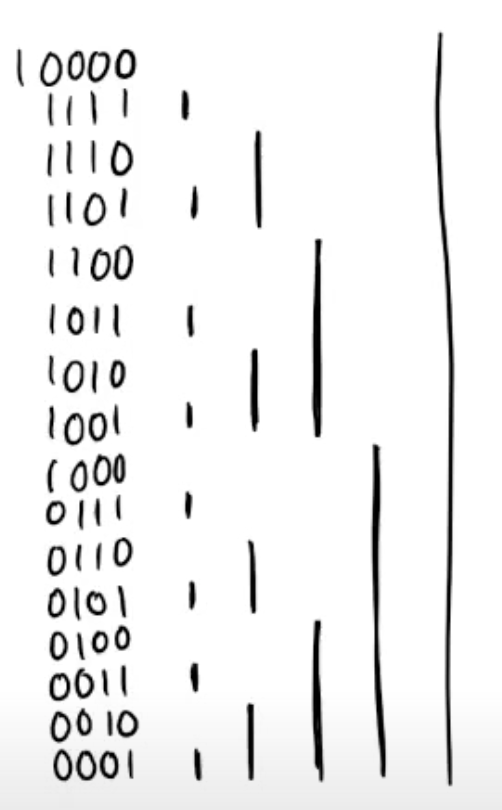
\includegraphics[width=0.15\textwidth]{femwickTree.png}
    \end{center}
    So you'll notice it is organized by lowest 1 (range of responsible). But there is some redundancy since some values are taken care by multiple others. 
    \subsection{Prefix Sums}
      We start at the current cell and staircase down until there are no bits left. How come?
      \begin{itemize}
        \item Suppose we start at position $11 = 1011_2$.
        \item Then we remove their smallest 1 bit and we are left with $1010_2 = 10$.
        \item We repeat the same process $1000_2=8$
        \item And we compute the sum of all these. And that will be your prefix sum up to and including that point. 
      \end{itemize}
      \par The loop runs in at most the number of bits, and that is why the complexity is $O(\lg{n})$ so the complexity of sum got worse, but for the update, we can now do a \textit{straight line to the right and check all the values that we must update.}
      \begin{itemize}
        \item Suppose we update $9 = 1001_2$.
        \item Then we also have to update $1010_2 =10, 1100_2 = 12$ and $10000_2=16$
        \item All the one bits that have to get updated are the bits that were 0 in our original number.
      \end{itemize}
      \par How can we obtain these numbers? Well, add a $1$ to the smallest 1 bit that is available, that way they slide over. To do it we can:
      $$i\ AND\ (-i)$$
      This can be done so using 2s complement. You can also implement $LowestOneBit$.
    \subsection{Update}
      Update all the cells that "own" the position, which are the ones that have $1$ on a bit that we don't have on.\par
      The loop will run exactly the number of off bits that we have, so it is bounded by $O(\lg{n})$.\par
      \textbf{Very simple to implement.}
    \subsection{Problems in which they come in handy}
      \subsubsection{Counting Inversions}
        Remember that an inversion in a subsequence is an index that is previous to another but its value is higher.\par
        In this case we must keep some sort of "running sum" of my inversions. \textit{So how many elements behind me pair with me?}.
        \begin{itemize}
          \item We have an array which stores what the prefix sum will be for the Fenwick Tree. Initially is all 0s.
          \item So we iterate with  $i$ and ask, for every single value, how many things are of that value behind me.
          \item We also keep a running sum of my inversions.
          \item So basically whenever we get a value, we want to get the sum of everything above it (which can be done with two calls to the Fenwick Tree), then we add the results to a running sum.
        \end{itemize}
        \par The drawing from the lecture explains it quite well.
        \begin{center}
          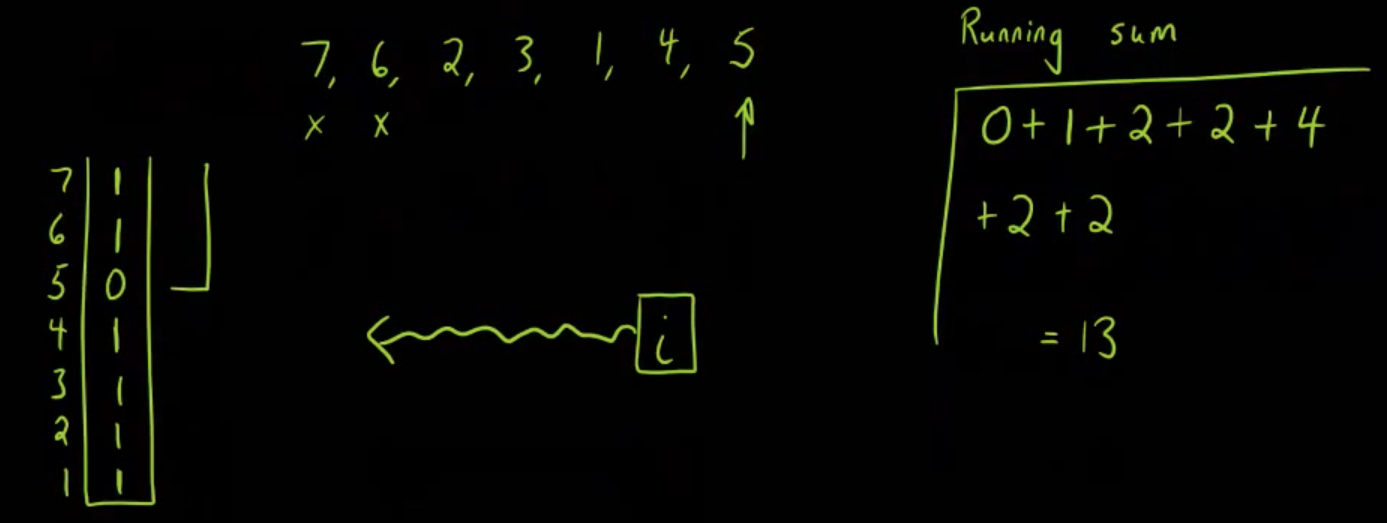
\includegraphics[width = 0.45\textwidth]{ftExample.png}
        \end{center}
        \par Reviewing, there are $n$ possible positions on that array, and the second is well obtaining the sum of everything above it in the data structure which is $n\lg{n}$ in the end.
      \subsubsection{Find $k^{th}$ tallest}
        You are given a listing of heights $[1,10^6]$. And there can be a random number of people from each height. You need to find the $k^{th}$ tallest. The types of queries are:
        \begin{itemize}
          \item \texttt{update h \#}, where you receive a certain height and update the quantity of people from that height. 
          \item \texttt{query k} find the $k^{th}$ tallest person.
        \end{itemize}
        \par Let's store a Fenwick tree for all possible heights. \textbf{Doesn't matter if some of them are empty}. You'll notice that by the end of the updates there might be some blank cells. Since it only saves aggregates for the ranges. 
        \begin{itemize}
          \item Let's say we want to find the $k^{th}$ element now. 
          \item Look for the largest power of 2 in my table and I do a high-low search on it. In this example it is 16, and the aggregate was too much, we need to look below me now.  
          \item We go to the next power of 2 and check the value (very similar to a binary search). 
          \item If we go too low, we substract the power of two from the number we are searching, and we know that our answer will be between the powers of two that we were searching for. 
        \end{itemize}
        \par This is again better understood with the drawing from the lecture.
        \begin{center}
          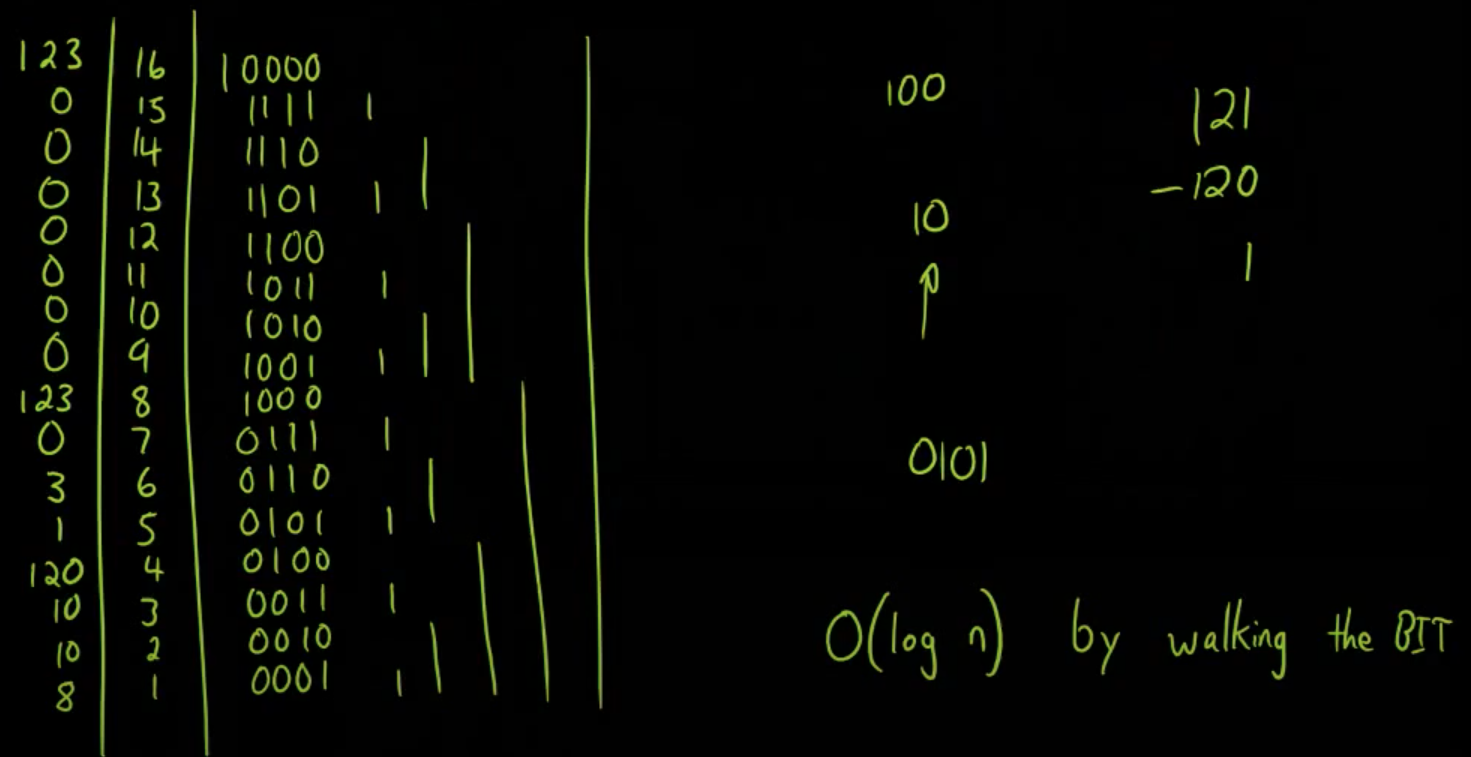
\includegraphics[width=0.45\textwidth]{kHeight.png}
        \end{center}
        \par By walking down the BIT the execution time is $O(\lg{n})$ since it is similar to binary search. 
      \subsubsection{Backwords BIT}
        In this case we want to update a range from $a$ to $b$ inclusive and tell me what is the given position for that value.\par
        No need to modify the BIT, as it can be used as a black box. So instead of storing information on the location we are gonna store information based in the change in value. So in the Fenwick tree, what we do when we receive an update for $a,b$
        \begin{itemize}
          \item We add the update value to the position $a$
          \item In the immediate succesor of $b$, we substract the same value.
        \end{itemize}
        \par And that way if we obtain the prefix sum will obtain me the value. And then the negative that we added will cancel that out for the rest of the values.\par
        \textbf{Big Note: Check the codes of the lecture, even though they are in Java, they might come in really handy.}
  \section{Emaxx - Fenwick Tree}
    Being $f$ a reversible function (you can determine input from output) and $A$ an array of $N$ numbers, a Fenwick Tree:
    \begin{itemize}
      \item Calculates the value of $f$ in range $[l,r]$ ($f(A_l,\ldots,A_r)$) in $O(\lg{n})$.
      \item Updates the value of an element of $A$ in $O(\lg{n})$
      \item Requires $O(N)$ memory
    \end{itemize}
    \par Also called Binary Indexed Trees (BIT). Most common use is sum of a range $f(A_1,A_k)=A_1,\ldots,A_k$.
    \subsection{Description}
      \subsubsection{Overview}
        Suppose the sum function. Given $A[0\ldots N-1]$. So the tree $T[0\ldots N-1]$ has each element equal to the sum of elements $A$ in some range $[g(i),i]$.
        $$T_i=\sum_{j=g(i)}^i A_j$$
        \par Where $0\leq  g(i)\leq i$ is satisfied. Unlike a regular "tree" we just need to mantain $T$ to handle all queries.\par
        How to get the sum of items of $A[0,r]$ and update some element in $A$
        \begin{lstlisting}
sum(r):
  res = 0 
  while (r >= 0):
    res += t[r]
    r = g(r) - 1 
  return res

increase(i, delta):
  for all j with g(j) <= i <= j:
    t[j] += delta // This is kind of the important part
        \end{lstlisting}
        \par The steps can be seen as:
        \begin{enumerate}
          \item Add the sum of range [g(r),r] to the result.
          \item Jumps to the range [g(g(r)-1),g(r)-1] and adds it.
          \item Repeats the process until it jumps from $[0,g(g(\ldots g(r)-1\ldots-1)-1)]$ to $[g(-1),-1]$, which is outside of the range
        \end{enumerate}
        The function increase works fairly similar.
        \begin{enumerate}
          \item Sums the ranges $[g(j),j]$ that satisfy $g(j)\leq i \leq j$ are increased by delta. We updates all elements in $T$ that correspond to ranges $A_i$
        \end{enumerate}
        \par Since both functions depend on $g(i)$ it is important to choose a special definition that handles the sums and update in $O(\lg{n})$ time.
      \subsubsection{Definition of $g(i)$}
        We replace all the last $1$ bits in the binary representation of $i$ with $0$. For example:
        $$g(11)=g(1011_2)=1000_2=8$$
        $$g(12)=g(1100_2)=1100_2=12$$
        $$g(15)=g(1111_2)=0000_2=0$$
        \par The trivial implementation is:
        $$g(i)=i\ AND\ (i+1)$$
        \par Now we iterate over all $j$ such that $g(j)\leq i \leq j$. Can be done so by starting at $i$ and flip the last unset bit, for example:
        $$10=0001010_2$$
        $$h(10)=11=0001011_2$$
        $$h(11)=15=0001111_2$$
        $$h(15)=31=0011111_2$$
        $$\vdots$$
        \par Can also be expressed as $h(j) = j\ OR\ (j+1)$
    \subsection{Implementation}
      \subsubsection{Finding sum in 1D array}
        Since the regular tree can only answer for $[0,r]$ we can obtain $[l,r]=[0,r]-[0,l-1]$. The Fenwick tree can be filled with 0s, or converted from an array.
        \begin{lstlisting}
struct FenwickTree {
  vector<int> bit;  // binary indexed tree
  int n;
  FenwickTree(int n) {
      this->n = n;
      bit.assign(n, 0);
  }
  FenwickTree(vector<int> a) : FenwickTree(a.size()) {
      for (size_t i = 0; i < a.size(); i++)
          add(i, a[i]);
  }
  int sum(int r) {
      int ret = 0;
      for (; r >= 0; r = (r & (r + 1)) - 1)
          ret += bit[r];
      return ret;
  }
  int sum(int l, int r) {
      return sum(r) - sum(l - 1);
  }
  void add(int idx, int delta) {
      for (; idx < n; idx = idx | (idx + 1))
          bit[idx] += delta;
  }
};
        \end{lstlisting}
        \par \textit{Note: at the moment of writing this I am using the BIT mostly as a black-box by coach suggestion.}
      \subsubsection{Finding minimum of $[0,r]$ in 1D array}
        Significant limitations since there is no way to obtain $min[l,r]$ since the queries are $[0,r]$ and teach time a value is updatedd, the new value has to be smaller than the current one. The min function is not a reversible one.
        \begin{lstlisting}
struct FenwickTreeMin {
  vector<int> bit;
  int n;
  const int INF = (int)1e9;
  FenwickTreeMin(int n) {
      this->n = n;
      bit.assign(n, INF);
  }
  FenwickTreeMin(vector<int> a) : FenwickTreeMin(a.size()) {
      for (size_t i = 0; i < a.size(); i++)
          update(i, a[i]);
  }
  int getmin(int r) {
      int ret = INF;
      for (; r >= 0; r = (r & (r + 1)) - 1)
          ret = min(ret, bit[r]);
      return ret;
  }
  void update(int idx, int val) {
      for (; idx < n; idx = idx | (idx + 1))
          bit[idx] = min(bit[idx], val);
  }
};
        \end{lstlisting}
        \par Can also be done to manage arbittrary min range queries and updates, but erquires a second BIT with different structure.
      \subsubsection{Finding sum in 2D Array}
        Very easy similar approach.
        \begin{lstlisting}
struct FenwickTree2D {
  vector<vector<int>> bit;
  int n, m;

  // init(...) { ... }

  int sum(int x, int y) {
      int ret = 0;
      for (int i = x; i >= 0; i = (i & (i + 1)) - 1)
          for (int j = y; j >= 0; j = (j & (j + 1)) - 1)
              ret += bit[i][j];
      return ret;
  }

  void add(int x, int y, int delta) {
      for (int i = x; i < n; i = i | (i + 1))
          for (int j = y; j < m; j = j | (j + 1))
              bit[i][j] += delta;
  }
};
        \end{lstlisting}
      \subsubsection{One based indexed approach}
        \textbf{Check the actual implementation in the source if you are locked to a 1-based indexed language. Otherwise...}
    \subsection{Range Operations}
      The operations supported by the tree are:
      \begin{itemize}
        \item Point Update and Range Query: just the same as explained before.
        \item Range Update and Point Query
        \item Range Update and Range Query
      \end{itemize}
      \subsubsection{Range Update and Point Query}
        Let the Fenwick tree start with 0s. Suppose we increase the interval $[l,r]$ by $x$. Two operations are done $add(l,x), add(r+1,-x)$.\par
        To obtain the value of $A[i]$, we take the prefix sum usinng the ordinary range sum method.  If $i<l$ then the two upadte operations have no effect annd the sum is $0$, if $i\in[l,r]$, then we get the answer $x$. If $i>r$ the second update cancels the effect of the first one.\par
        This is a one-based indexed implementation.
        \begin{lstlisting}
void add(int idx, int val) {
  for (++idx; idx < n; idx += idx & -idx)
      bit[idx] += val;
}
void range_add(int l, int r, int val) {
  add(l, val);
  add(r + 1, -val);
}
int point_query(int idx) {
  int ret = 0;
  for (++idx; idx > 0; idx -= idx & -idx)
      ret += bit[idx];
  return ret;
}
        \end{lstlisting}
      \subsubsection{Range Updates and Queries}
        We use 2 BITs initialized with 0s.\par
        The process to increment the interval $[l,r]$ by $x$ is now:
        \begin{lstlisting}
def range_add(l, r, x):
  add(B1, l, x)
  add(B1, r+1, -x)
  add(B2, l, x*(l-1))
  add(B2, r+1, -x*r))
        \end{lstlisting}
        \par After the update the query returns the following values for $sum[0,i]$
        $$0\text{ if $i<l$}$$
        $$x*(i-(l-1))\text{ if $l\leq i\leq r$}$$
        $$x*(r-l+1)\text{ if $i > r$}$$
        \par We canwrite therangesum as diffeerence of two terms, $B_1$ for the first and $B_2$ for the second.
        $$sum[0,i]=sum(B_1,i)*i-sum(B_2,i)$$
        $$=0*i-0\text{ if $i<l$}$$
        $$=x*i-x*(l-1)\text{ if $l\leq i\leq r$}$$
        $$=0*i-(x*(l-1)-x*r)\text{ if $i > r$}$$
        \par Arbitrary range sums can be obtained with thee prefix sums for $l-1$ and $r$ and taking their difference.
        \begin{lstlisting}
def add(b, idx, x):
  while idx <= N:
      b[idx] += x
      idx += idx & -idx
def range_add(l,r,x):
  add(B1, l, x)
  add(B1, r+1, -x)
  add(B2, l, x*(l-1))
  add(B2, r+1, -x*r)
def sum(b, idx):
  total = 0
  while idx > 0:
      total += b[idx]
      idx -= idx & -idx
  return total
def prefix_sum(idx):
  return sum(B1, idx)*idx -  sum(B2, idx)
def range_sum(l, r):
  return prefix_sum(r) - prefix_sum(l-1)
        \end{lstlisting}
  \section{Fenwick Tree Range Updates}
    Allows 2 operations on an array, increment a value by a given amount, and find the sum of a segment in $O(\lg{n})$ time. Array of the same size being updated and queries.\par
    Initial implementation:
    \begin{lstlisting}
private void update(int at, int by) {
  while (at < data.length) {
    data[at] += by;
    at |= (at + 1);
  }
}
    
private int query(int at) {
  int res = 0;
  while (at >= 0) {
    res += data[at];
    at = (at & (at + 1)) - 1;
  }
  return res;
}
    \end{lstlisting}
    \par $query(at)$ returns the sum of all elements up to $at$. For an arbitrary segment $query(right)-query(left-1)$ can be done.\par
    The regular tree only supports updating one element at a time, but to do \textbf{each value between $l,r$} we can modify them.\par
    The following code is supposedly untested according to the author but he hopes it works.
    \begin{lstlisting}
private void update(int left, int right, int by) {
  internalUpdate(left, by, -by * (left - 1));
  internalUpdate(right, -by, by * right);
}
    
private void internalUpdate(int at, int mul, int add) {
  while (at < dataMul.length) {
    dataMul[at] += mul;
    dataAdd[at] += add;
    at |= (at + 1);
  }
}
    
private int query(int at) {
  int mul = 0;
  int add = 0;
  int start = at;
  while (at >= 0) {
    mul += dataMul[at];
    add += dataAdd[at];
    at = (at & (at + 1)) - 1;
  }
  return mul * start + add;
}
    \end{lstlisting}
    \par We implement a Fenwick tree via a normal (point-update) one that stores linear functions instead of values.
  \begin{thebibliography}{}
    \bibitem{alive}
      \textit{Episode 0 - Fenwick Trees},
      Algorithms Live!
      From: https://www.youtube.com/watch?v=kPaJfAUwViY
    \bibitem{top}
      \textit{Fenwick Tree},
      CP-Algorithms,
      From: https://cp-algorithms.com/data\_structures/fenwick.html 
    \bibitem{petr}
      \textit{Fenwick tree range updates},
      Algorithms Weekly by Petr Mitrichev,
      From: https://petr-mitrichev.blogspot.com/2013/05/fenwick-tree-range-updates.html
  \end{thebibliography}
\end{document}